\documentclass[12pt,a4paper]{article}
\usepackage[utf8]{inputenc}
\usepackage[T1]{fontenc}
\usepackage{parskip}

\usepackage{graphicx}
\usepackage{media9}
\title{Using media9 to include video and audio files}
\begin{document}

Videos and audios don't play on Overleaf! Download the PDF and open in Acrobat Reader to view. :-)

This is an .mp4 file:

% using a .mp4; downloaded from https://www.youtube.com/watch?v=-9iXD2-hbJM
\includemedia[width=0.6\linewidth,height=0.6\linewidth,activate=pageopen,
passcontext,
transparent,
addresource=penguinschasingbutterfly.mp4,
flashvars={source=penguinschasingbutterfly.mp4}
]{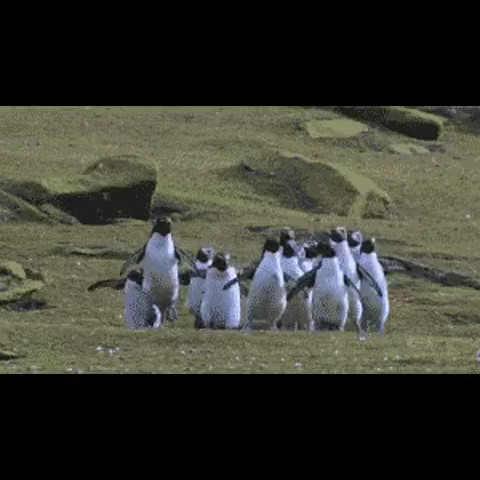
\includegraphics[width=0.6\linewidth]{penguins}}{VPlayer.swf}

This is a YouTube video (needs an Internet connection to view):

% using a YouTube video
\includemedia[
  width=0.6\linewidth,height=0.3375\linewidth,
  activate=pageopen,
  flashvars={
  modestbranding=1 % no YT logo in control bar
  &autohide=1 % controlbar autohide
  &showinfo=0 % no title and other info before start
  &rel=0 % no related videos after end
}
]{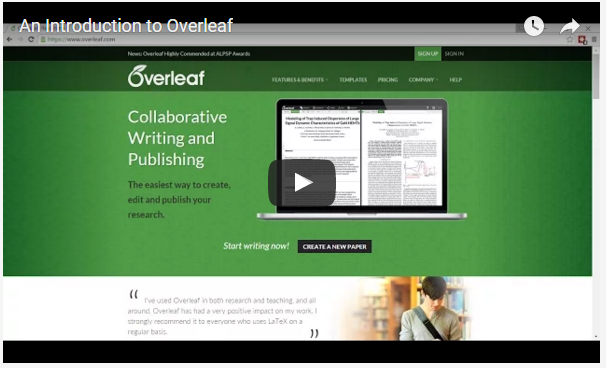
\includegraphics[width=0.6\linewidth]{048}}{https://www.youtube.com/v/g8Ejj0T0yG4?rel=0}

This is an .mp3 file:
%% MP3 downloaded from https://www.sample-videos.com/download-sample-audio.php
\includemedia[
  transparent,
  passcontext,
  addresource=SampleAudio.mp3,
  flashvars={source=SampleAudio.mp3},
]{\color{blue}\framebox[0.4\linewidth][c]{Applause}}{APlayer.swf}
\end{document}
